\section{Problem 4}\label{prob4}

The overall algorithm for the global snapshot consists of three main steps:
\begin{enumerate}
    \item \textbf{Spanning Tree Construction}
    \item \textbf{Recording Snapshots at Each Node}
    \item \textbf{Propagating Snapshots to the Root Node through the Spanning Tree}
\end{enumerate}

\subsection{Spanning Tree Construction}
For constructing the spanning tree, we use the algorithm discussed in question \ref{prob3}, with slight modifications to leverage the synchronous nature of the links and reduce the number of messages. Specifically:
\begin{itemize}
    \item The \texttt{REJ} message is eliminated, and instead, a timeout mechanism is employed to detect cases where a node has already been connected to a parent.
    \item Further optimization, such as eliminating the \texttt{ACK} message, could be achieved if the network's diameter were known. While a bound on the diameter can be indirectly derived as \(n-1\) (given a bound on the number of nodes \(n\)), we skip this optimization as it is not explicitly stated in the problem.
\end{itemize}

\noindent The modified algorithm for constructing the spanning tree is as follows:

Each node in the network stores the following information:
\begin{itemize}
    \item \textbf{Parent:} Initialized to \texttt{null}. (The parent node in the spanning tree.)
    \item \textbf{Children:} Initialized to an empty list. (The list of children in the spanning tree.)
    \item \textbf{ACK Count:} Initialized to \texttt{0}. (The number of acknowledgments received from children \(c\) indicating that the spanning tree construction is complete for the subtree rooted at \(c\).)
\end{itemize}

There are three types of messages in the protocol: \texttt{ASK}, \texttt{CHILD}, and \texttt{ACK}. Each node follows the rules below for handling each message type:

\subsubsection{Message Handling Rules}

\paragraph{On receiving an \texttt{ASK} message:}
\begin{enumerate}
    \item If the \texttt{Parent} is not \texttt{null}: (The node is already connected to a parent.)
    \begin{itemize}
        \item Ignore the message. (No action is taken. The rejection is implicit because of timeout.)
    \end{itemize}
    \item Otherwise:
    \begin{itemize}
        \item Set the \texttt{Parent} to the sender. (The node accepts the sender as its parent.)
        \item Send a \texttt{CHILD} message to the sender. (The sender is accepted as a child.)
        \item Send a \texttt{ASK} message to all other neighbors, excluding the sender. Start a timer for the \texttt{ASK} message with duration \(2\times T\). (The node ask its neighbors to become its children. It also sets a timer with maximum round-trip time. Any node not responding within this time to the \texttt{ASK} message does not become a child.)
    \end{itemize}
\end{enumerate}

\paragraph{On receiving a \texttt{CHILD} message:}
\begin{enumerate}
    \item Add the sender to the \texttt{Children} list. (The node accepted a child.)
    \item If \(\texttt{ACK Count} = \texttt{Children.size()}\) and the timer has expired: (All children have informed the node that the spanning tree construction is complete for their subtrees and the timer has expired)
    \begin{itemize}
        \item Send an \texttt{ACK} message to the parent. (All children have acknowledged.)
    \end{itemize}
\end{enumerate}

\paragraph{On receiving an \texttt{ACK} message:}
\begin{enumerate}
    \item Increment the \texttt{ACK Count} by \texttt{1}. (The node received an acknowledgment from a child indicating that the spanning tree construction is complete for the subtree rooted at the child.)
    \item If \(\texttt{ACK Count} = \texttt{Children.size()}\) and the timer has expired: (All children have acknowledged and the timer has expired)
    \begin{itemize}
        \item Send an \texttt{ACK} message to the parent. (Send an acknowledgment to the parent indicating that the spanning tree construction is complete for the subtree rooted at the node.)
    \end{itemize}
\end{enumerate}

\subsubsection{Timeout Handling}
If the timer for the \texttt{ASK} message expires, the node proceeds as follows: (Within, this time, the node expects a \texttt{CHILD} message from the neighbor which has accepted the node as a parent.)
\begin{enumerate}
    \item If \(\texttt{ACK Count} = \texttt{Children.size()}\): (All children have acknowledged that the spanning tree construction is complete for their subtrees.)
    \begin{itemize}
        \item Send an \texttt{ACK} message to the parent. (Send an acknowledgment to the parent indicating that the spanning tree construction is complete for the subtree rooted at the node.)
    \end{itemize}
\end{enumerate}

\subsubsection{Initialization and Termination Conditions}
A node \(i\) begins the spanning tree construction by:
\begin{itemize}
    \item Sending an \texttt{ASK} message to all its neighbors. (The node asks its neighbors to become its children.)   
    \item Setting itself as the root node for its local state. (The node is the root of the spanning tree.)
    \item Starting a timer for the \texttt{ASK} message with a duration of \(2 \times T\). (The node sets a timer with maximum round-trip time. Any node not responding within this time to the \texttt{ASK} message does not become a child.)
\end{itemize}

The spanning tree construction is considered complete at node \(i\) when the following conditions are met:
\begin{itemize}
    \item The \texttt{ACK Count} equals the size of its \texttt{Children} list. (All children have acknowledged that the spanning tree construction is complete for their subtrees.)
    \item The timer has expired. (The timer for the \texttt{ASK} message has expired.)
\end{itemize}

\subsection{Recording Snapshots at Each Node}

To record snapshots at each node, we modify the Chandy-Lamport algorithm to handle non-FIFO channels. To do this, we introduce a delay after sending the marker message to ensure that all messages sent before the marker message are received.

Each node in the network maintains the following information:

\begin{itemize}
    \item \textbf{Local State:} Stores the state of the node, initially set to \texttt{null}.
    \item \textbf{Channel States:} For each neighbor, stores the state of the channel directed to the node. Specifically, for each neighbor \(j\), the node maintains the state of the channel from \(j\) to itself. All channel states are initialized to \texttt{null}.
\end{itemize}

When node \(x\) receives a marker message from a neighbor \(y\) along the channel \(y \rightarrow x\), the following steps are executed:

\begin{enumerate}
    \item \textbf{If the node has not recorded its local state:}
    \begin{itemize}
        \item Upon receiving the marker message, wait for \(T\) time units to detect any pending messages. If any pending messages are detected, process them and accordingly update the local state. (This step ensures that all messages sent before the marker message are received and processed.)
        \item Record the local state of the node as the state at the end of the waiting period. Record the state of the channel \(y \rightarrow x\) as empty. (The channel state is recorded as empty since the marker message is the last message sent along the channel.)
        \item Send marker messages to all neighbors. (The node sends marker messages to all neighbors asking them to record their local states.)
        \item After sending the marker messages, delay sending any further messages for \(2 \times T\) time units, i.e., wait for \(2 \times T\) time units before placing any new messages in the channels. (This delay ensures that the receiving node can differentiate between messages sent before and after the marker message.)
    \end{itemize}
    
    \item \textbf{If the node has already recorded its local state:}
    \begin{itemize}
        \item Let \(M_1\) denote the set of messages received before the marker message from \(y\) and after the local state was recorded by \(x\). (These messages are received after the local state was recorded but before the marker message was received.)
        \item Upon receiving the marker message, the node waits for \(T\) time units to detect any pending messages. Let \(M_2\) represent the set of messages received during this waiting period from \(y\). (These messages are received after the marker message was received and during the waiting period.)
        \item Record the state of the channel \(y \rightarrow x\) as \(M_1 \cup M_2\), the union of the two sets of messages. 
    \end{itemize}
\end{enumerate}

In order to see how we use the timeouts value to differentiate between messages sent before and after the marker message, consider the following scenario:(All the time values are with respect to a global reference clock.)

A node $x$ sends a marker message $M$ to a neighbor $y$ at time $t_M = t_1$. The message is received by $y$ at time $t_{rec}^{(M)} \in [t_1, t_1+T]$. Since our algorithm does not restrict sending messages before the marker, assume that $x$ sent another message $msg$ to $y$ at time $t_{msg} = t_1 - \epsilon$, where $\epsilon$ is a small positive value. This message is received by $y$ at time $t_{rec}^{(msg)} \in [t_1 - \epsilon, t_1 + T - \epsilon]$. In the worst case, it is possible that $t_{rec}^{(M)} = t_1$ while $t_{rec}^{(msg)} = t_1 + T - \epsilon$. As a result, after receiving the marker message, $y$ must wait for $T$ time units to detect any pending messages.

% Inserting the figure
\begin{figure}[h]
    \centering
    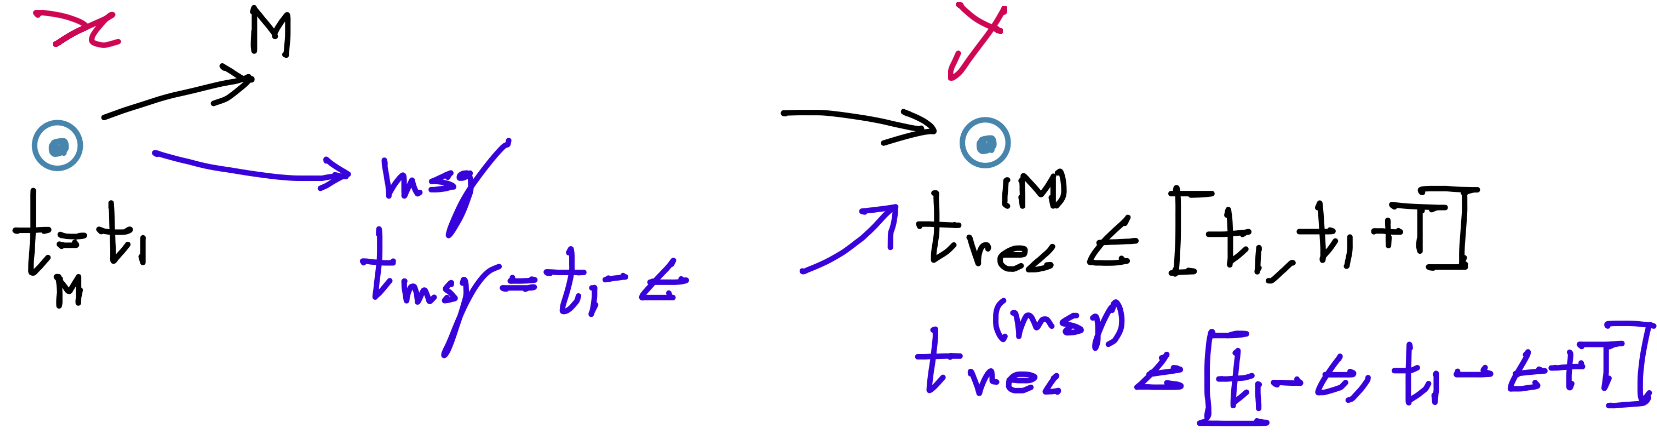
\includegraphics[width=0.8\textwidth]{IMG/Q4.jpeg}
    \caption{Illustration of the timeout mechanism for recording snapshots}
    \label{fig:fig1}
\end{figure}

Since $y$ is unaware of the delay for the marker message, it must wait $T$ time units irrespective of the marker's delay to detect any pending messages. If the marker message is delayed by $T$ time units, $y$ will still have to wait for $T$ time units to detect any pending messages after the marker's receive. In the worst case, $y$ may have to wait until $t_1 + 2T$ to identify any pending messages. After this period, any message received by $y$ is considered to have been sent after the marker message. This justifies our algorithm's requirement that $x$ must wait for $2 \times T$ time units before placing any new messages in the channel.


\subsubsection{Initialization and Termination Conditions}

The global snapshot algorithm is initiated by a node \(i\) through the following steps:
\begin{itemize}
    \item The node first records its local state.
    \item It then sends marker messages to all its neighbors.
    \item After sending the marker messages, the node waits for \(2 \times T\) time units before placing any new messages in the channel.
\end{itemize}


A local state recording of a node is deemed complete when both the node's state and all its incoming channel states have been recorded. This condition will eventually be satisfied for all nodes in the network, as the graph is connected. 

At this stage, we will not detect the completion of the global snapshot but we note here that each node can independently detect the completion of its local snapshot recording. We will now use the spanning tree constructed in the previous step to propagate the snapshots to the root node.

\subsection{Propagating Snapshots to the Root Node through the Spanning Tree}
As we noted, every node can independently detect the completion of its local snapshot recording. The next step is to propagate the snapshots to the root node through the spanning tree. The idea is to send the snapshots from the leaf nodes to the root node, merging the snapshots as they propagate upwards. A node can send the snapshot to its parent only when it has received snapshots from all its children and has recorded its local state. The message format can be defined as follows where we assume that the snapshot is a JSON object: (The format of the snapshot can be modified based on the requirements of the application. The only requirement is that the receiver and sender agree on the format.)

\begin{verbatim}
{
    "node_id": <node_id>,
    "local_state": <local_state>,
    "channel_states": {
        "link_1": <state>,
        "link_2": <state>,
        ...
    }
}
\end{verbatim}

Each node \(j\) in the network maintains the following information:
\begin{itemize}
    \item \textbf{Snapshot State:} Initially set to \texttt{null}.
    \item \textbf{Received Snapshots:} A list of snapshots received from all children, initially set to an empty list.
\end{itemize}

When node \(j\) receives a snapshot from a child \(i\) or detects that its local state and channel states have been recorded, it follows the steps below:

\begin{enumerate}
    \item If the snapshot is received from a child \(i\), add it to the \texttt{Received Snapshots} list. (The snapshot received from child \(i\) is added to the list of received snapshots.)
    \item If the size of the \texttt{Received Snapshots} list equals the number of children of node \(j\), and the local state and channel states of node \(j\) have been recorded: (All children have sent snapshots from their subtrees, and the local state and channel states of node \(j\) have been recorded.)
    \begin{itemize}
        \item Merge the local state of node \(j\) with the channel states of node \(j\), along with the snapshots received from all children. (The local state and channel states of node \(j\) are merged with the snapshots received from all children.)
        \item Send the merged snapshot to the parent of node \(j\). (The merged snapshot is sent to the parent of node \(j\).)
    \end{itemize}
\end{enumerate}

The node \(i\) that initiated the global snapshot can detect its completion once it receives a snapshot from all its children in the spanning tree. The snapshot received by the root node is the global snapshot of the network.

\subsection{Message Complexity}

Let \(n\) be the number of nodes in the network and \(m\) be the number of channels. The message complexity of the global snapshot algorithm can be analyzed as follows:

\begin{enumerate}
    \item \textbf{Spanning Tree Construction:} During the spanning tree construction, each node sends at most one \texttt{ASK} message to each of its neighbors. This results in atmost \(2 \times m\) messages. Additionally, the \texttt{CHILD} and \texttt{ACK} messages are sent in response from child to parent, each being sent \(n-1\) times. Therefore, the total number of messages sent during spanning tree construction is:
    \[
    2 \times (m + n - 1)
    \]
    
    \item \textbf{Recording Snapshots at Each Node:} The marker message is sent along each channel at most twice, so the number of messages sent during snapshot recording is at most:
    \[
    2 \times m
    \]
    
    \item \textbf{Propagating Snapshots to the Root Node:} The number of messages sent during the propagation of snapshots to the root node is \(n-1\).
\end{enumerate}

Summing the message complexities of these three steps, the total message complexity of the global snapshot algorithm is:
\[
2 \times (m + n - 1) + 2 \times m + (n - 1) = 4 \times m + 3 \times n - 3 = O(m + n)
\]

